% Generated by Sphinx.
\def\sphinxdocclass[english]{xmosmodern}
\documentclass[  collection]{xmosmodern}
\usepackage[utf8]{inputenc}
\DeclareUnicodeCharacter{00A0}{\nobreakspace}

\usepackage{longtable}



\title{Serial to Ethernet bridging application manual}
\date{June 06, 2014}
\author{}
\newcommand{\sphinxlogo}{}
\newcommand{\releasename}{Release}
\usepackage{xsphinx}
\usepackage{threeparttable}
\usepackage{fancyvrb}
\usepackage{indent}
\renewcommand\bfcode\textbf
\renewcommand\bf\textbf
\graphicspath{{./}{./images/}}
\makeindex

\newcommand\PYGZat{@}
\newcommand\PYGZlb{[}
\newcommand\PYGZrb{]}

\setlength{\emergencystretch}{8em}
\FourDigitsInTocSection
\start

\maketitle
\pretoc
\phantomsection\label{index::doc}

%summary!

% NON-FULLWIDTH SECTION



% NON-FULLWIDTH SECTION
\clearpage
\chapter{Application Overview}
\label{overview::doc}\label{overview:serial-to-ethernet-bridging-application-manual}\label{overview:application-overview}%summary!
\begin{inthisdocument}
\item \nameref{overview:introduction}
\item \nameref{overview:feature-list}
\end{inthisdocument}




% NON-FULLWIDTH SECTION
\section{Introduction}
\label{overview:introduction}

The Serial to Ethernet application (referred to as S2E) firmware serves as a reference design to add Ethernet connectivity to any serial device. The solution offers flexibility in configuring multiple UART devices (up to 8 UARTs) to bridge them to Ethernet networks. Design utilizes some of the existing XMOS xSOFTip components to implement Ethernet MAC, TCP/IP and multiUART functionality.


The firmware mainly functions as bridge between serial and Ethernet data communication end points. This application includes a telnet server in order to facilitate data communication from host applications via separate telnet sockets for each of the configured UARTs. It also provides an embedded web server and a dedicated telnet socket for UART configuration management. UDP mode device discovery feature is provided in order to discover and configure the S2E devices available in the network.



% NON-FULLWIDTH SECTION
\section{Feature list}
\label{overview:feature-list}


% NON-FULLWIDTH SECTION
\subsection{Supported}
\label{overview:supported}\begin{itemize}
\item   10/100 Mbit Ethernet port

\item   Supports up to 8 serial ports at the following baud rates: 115200, 57600, 38400,
28800, 19200, 14400, 9600, 7200, 4800, 2400, 1200, 600, 300, 150

\item   Supports various parity mode, character length, start/stop bit

\item   Device discovery and device IP configuration management using UDP

\item   Web page for UART configuration

\item   Telnet server functionality: supports data transfer via telnet socket for each UART

\item   Flash support for IP and UART configuration, web page storage and retrieval

\item   Telnet mode UART configuration support

\item   CMOS/TTL level and RS232 level communication for UARTs

\item   All the 8 UARTs can be configured in different configurations

\end{itemize}




% NON-FULLWIDTH SECTION
\subsection{Not supported}
\label{overview:not-supported}\begin{itemize}
\item   UART to UART communication (serial extender or pair configuration)

\item   UDP mode data transfer

\item   VirtualCOM port for the UARTs for Configuration

\end{itemize}




% NON-FULLWIDTH SECTION
\clearpage
\chapter{Hardware platforms}
\label{hardware_platform:hardware-platforms}\label{hardware_platform::doc}%summary!
\begin{inthisdocument}
\item \nameref{hardware_platform:hardware-requirements}
\item \nameref{hardware_platform:hardware-setup}
\end{inthisdocument}




% NON-FULLWIDTH SECTION
\section{Hardware requirements}
\label{hardware_platform:hardware-requirements}\begin{description}
\item[This application runs on an L2 device on the sliceKIT core board. Following hardware is required for running this application:]\begin{itemize}
\item   xCORE General Purpose (L-series) sliceKIT core board 1V2 (XP-SKC-L2)

\item   Ethernet sliceCARD 1V1 (XA-SK-E100)

\item   Multi UART sliceCARD (XA-SK-UART-8)

\item   xTAG-2 debug adapter and sliceKIT connector (xTAG-2 and XA-SK-XTAG2)

\item   Ethernet cable

\item   Power supply 12V

\end{itemize}


\end{description}




% NON-FULLWIDTH SECTION
\section{Hardware setup}
\label{hardware_platform:hardware-setup}

MultiUART component requires 8-bit ports for both transmit and receive ports. The current version of the \emph{Serial to Ethernet} application runs on a two tile device. The sliceCARDs should be connected to the sliceKIT core board in the following manner:

\begin{tabular}{lll}
\Toprule
\textbf{\textbf{sliceCARD}} & \textbf{\textbf{sliceKIT Connector}} & \textbf{\textbf{sliceKIT - Jumper}}\\
\midrule
Ethernet & Triangle & J5\\
MultiUART & Square & J8\\
\bottomrule
\end{tabular}

\begin{description}
\item[The Multi UART sliceCARD has two types of voltage levels of communications.]\begin{itemize}
\item   CMOS TTL

\item   RS-232

\end{itemize}


\end{description}



By default, Multi UART sliceCARD uses the RS-232 levels. In order to use the CMOS TTL levels, short J3 pins (25-26) of the Multi UART sliceCARD. Only one voltage level type can be used for all 8 UART channels (RS-232 or CMOS TTL). When using the RS-232 levels, UART device pins must be connected to J4 of the Multi UART sliceCARD. When using TTL levels, UART device pins must be connected to J3 of the Multi UART sliceCARD (along with J3 25-26 pins shorted). UART mapping information is as below:

\begin{tabular}{lll}
\Toprule
\textbf{\textbf{UART Channel}} & \textbf{\textbf{J3/J4 Pin no.(TX)}} & \textbf{\textbf{J3/J4 Pin no.(RX)}}\\
\midrule
0 & 1 & 2\\
1 & 5 & 6\\
2 & 7 & 8\\
3 & 11 & 12\\
4 & 13 & 14\\
5 & 17 & 18\\
6 & 19 & 20\\
7 & 23 & 24\\
\bottomrule
\end{tabular}

\begin{figure}[h]
\begin{sidecaption}{Hardware setup}

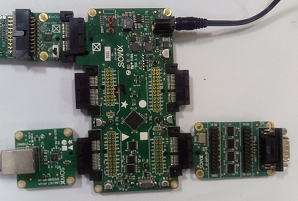
\includegraphics[width=0.500\linewidth]{hardware_setup.png}
\end{sidecaption}\end{figure} \DocumentFooterFix



% NON-FULLWIDTH SECTION
\clearpage
\chapter{System description}
\label{system_description:system-description}\label{system_description::doc}%summary!
\begin{inthisdocument}
\item \nameref{system_description:software-architecture}
\item \nameref{system_description:software-components-used}
\item \nameref{system_description:resource-usage}
\end{inthisdocument}



This section briefly describes the software components used, logical cores and resource usage details.



% NON-FULLWIDTH SECTION
\section{Software architecture}
\label{system_description:software-architecture}\begin{figure}[h]
\begin{sidecaption}{Core usage}

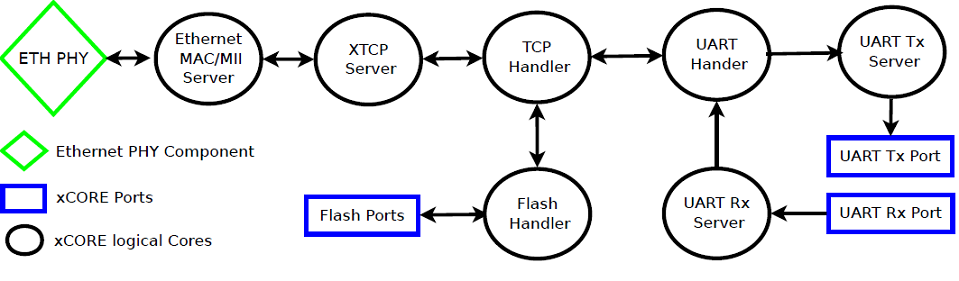
\includegraphics[width=\ScaleIfNeeded]{s2e_cores.png}
\end{sidecaption}\end{figure} \DocumentFooterFix


In order to achieve the desired data bridging, this application essentially maps each of the configured UART to a telnet socket and maintains application buffers (FIFOs) for each of such mapping. Whenever there is any UART data available, the \emph{UART Handler} core fills the appropriate UART Rx buffer and notifies \emph{TCP Handler} logical core to consume this data. Similarly whenever there is any Ethernet data from \emph{Ethernet MAC/MII server}, \emph{XTCP Server} logical core notifies \emph{TCP Handler} core, which acts as a TCP client about data availability. \emph{TCP Handler} stores this data into respective application buffers. This data is then consumed by \emph{UART handler} and then pushed to \emph{UART Tx ports} by \emph{UART TX server} logical core.



% NON-FULLWIDTH SECTION
\subsection{Cores}
\label{system_description:cores}

The design uses seven logical cores as described below.


The MultiUART component comprises two logical cores, one acting as a transmit (TX) server for up to 8 UARTs, and the other acting as a receive (RX) server for up to 8 UARTs.


UART\_handler is an application core that interfaces with the UART RX and TX servers. It handles UART configuration requests, facilitates to store the UART data received from UART RX server into respective application buffers and transfers the data received from TCP clients to UART TX server.


TCP\_Handler is another application core that initializes and manages the application. It interfaces with the flash module for UART configuration storage and recovery, handles all the xtcp application events (application data and UI configuration requests) received from the xtcp server module. UDP discovery management, web server handling, telnet data extraction are all implemented in this logical core.


The XTCP server runs on a single logical core and connects to the Ethernet MAC component which uses a single logical core. It uses XC channel to communicate to clients (TCP\_Handler in this case) using XTCP events.


The Flash core handles flash data sotrage and retrieval requests from TCP\_handler core based on the application dynamics such as start-up or UI driven requests.



% NON-FULLWIDTH SECTION
\subsection{Buffering}
\label{system_description:buffering}

Buffering for the TX server is managed by the UART\_handler Core. Data is transferred to the UART TX logical core via a shared memory interface.


There is no buffering provided by the UART RX server. The UART\_handler core is able to respond to the received data in real time and store them in buffer(s) available in the  TCP\_handler core via token notifcations.



% NON-FULLWIDTH SECTION
\subsection{Communication model}
\label{system_description:communication-model}

The \verb`sc_multi_uart` module utilises a combination of shared memory and channel communication. Channel communication is used on both the RX and TX servers to pause the logical core and subsequently release the logical core when required for reconfiguration. The primary means of data transfer for both the RX and TX logical cores is via shared memory. The RX logical core utilises a channel to notify any client (UART\_handler in this case) of available data - this means that events can be utilised within an application to avoid the requirement for polling for received data.


XTCP module and flash core connects to TCP\_handler client using their repective XC channels.



% NON-FULLWIDTH SECTION
\section{Software components used}
\label{system_description:software-components-used}
\begin{tabularx}{\linewidth}{lY}
\Toprule
\textbf{Component} & \textbf{Description}\\
\midrule
sc\_ethernet & Two logical core (lite) version of the ethernet component implementing 10/100 MII Ethernet MAC and filters\\
sc\_xtcp & Micro TCP/IP stack for use with sc\_ethernet component\\
sc\_multi\_uart & Component for implementing multiple serial device communication\\
sc\_util & General utility modules for developing for XMOS devices\\
sc\_website & Component framework for Embedded web site development\\
sc\_slicekit\_support & sliceKIT library to use L-series core board's flash for application\\
sc\_otp & Library for reading MAC from sliceKIT core board's OTP memory\\
\bottomrule
\end{tabularx}




% NON-FULLWIDTH SECTION
\section{Resource usage}
\label{system_description:resource-usage}

The overall platform usage and individual node usage shown in Figure~\ref{system_description:fig-resource-usage}. User can get this information on the \emph{Binary} window or by a \verb`double click` of the binary file present on the \emph{Binaries} folder in \emph{Project Explorer}, after compiling the application using \emph{xTIMEcomposer}.
\begin{figure}[h]
\begin{sidecaption}{Resource usage}[system_description:fig-resource-usage]

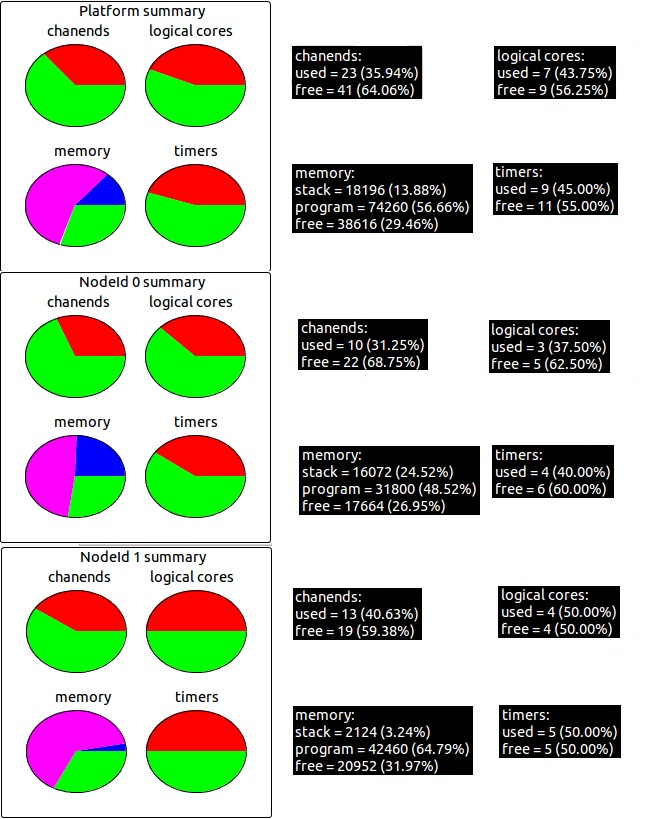
\includegraphics[width=\ScaleIfNeeded]{resource_usage.jpg}
\end{sidecaption}\end{figure} \DocumentFooterFix



% NON-FULLWIDTH SECTION
\clearpage
\chapter{Programming guide}
\label{programming_guide:programming-guide}\label{programming_guide::doc}%summary!
\begin{inthisdocument}
\item \nameref{programming_guide:getting-started}
\item \nameref{programming_guide:source-code-structure}
\item \nameref{programming_guide:notes-on-application-interfaces}
\end{inthisdocument}




% NON-FULLWIDTH SECTION
\section{Getting started}
\label{programming_guide:getting-started}


% NON-FULLWIDTH SECTION
\subsection{Installation of xTIMEcomposer Tools Suite}
\label{programming_guide:installation-of-xtimecomposer-tools-suite}

The Serial to Ethernet application requires xTIMEcomposer version 13.0.0 or greater. It can be downloaded at the following URL \parurl{http://www.xmos.com/support/xtools}
\begin{description}
\item[The following components are required to build the \emph{Serial to Ethernet application}:]\begin{itemize}
\item   sw\_serial\_to\_ethernet: git://github.com/xcore/sw\_serial\_to\_ethernet

\item   sc\_multi\_uart: git://github.com/xcore/sc\_multi\_uart.git

\item   sc\_xtcp: git://github.com/xcore/sc\_xtcp.git

\item   sc\_ethernet: git://github.com/xcore/sc\_ethernet.git

\item   sc\_util: git://github.com/xcore/sc\_util.git

\item   sc\_website: git://github.com/xcore/sc\_website.git

\item   sc\_slicekit\_support: git://github.com/xcore/sc\_slicekit\_support

\item   sc\_otp: git://github.com/xcore/sc\_otp

\end{itemize}


\end{description}



All these components are packaged as a software distribution. Once this zip file is selected, you can follow the below instructions to build and use the software.



% NON-FULLWIDTH SECTION
\subsubsection{Import and build procedure using xTIMEcomposer studio}
\label{programming_guide:import-and-build-procedure-using-xtimecomposer-studio}

To install the software, open the xTIMEcomposer (v13.0.0 or later) and follow these steps:
\begin{enumerate}
\item   Open the xTIMEcomposer studio.

\item   Open the \emph{Edit} perspective (Window -\textgreater{} Open Perspective -\textgreater{} XMOS Edit).

\item   Access the Import option either by right clicking the project in the project explorer window or through File -\textgreater{}Import menu

\item   Click \emph{Import} option in the \emph{Project Explorer} window (Import -\textgreater{} General -\textgreater{} Existing Projects into Workspace and click Next).

\item   Choose \emph{Select archive file} option and click \emph{Browse} button.

\item   Select s2e release zip file and click \emph{Finish} button

\item   The application is called as \emph{app\_serial\_to\_ethernet} in the \emph{Project Explorer} window.

\end{enumerate}



Build the \verb`serial to ethernet` application:
\begin{enumerate}
\item   Click on the \emph{app\_serial\_to\_ethernet} item in the \emph{Project Explorer} window.

\item   Click on the \emph{Build} (indicated by a `Hammer' picture) icon.

\item   Check the \emph{Console} window to verify that the application has built successfully.

\end{enumerate}




% NON-FULLWIDTH SECTION
\subsection{Flash the web pages and device configuration}
\label{programming_guide:flash-the-web-pages-and-device-configuration}

To flash the web pages and device configuration using xTIMEcomposer studio:
\begin{enumerate}
\item   In the \emph{Project Explorer} window, locate the \emph{app\_serial\_to\_ethernet.xe} and \emph{web\_data.bin} in the (app\_serial\_to\_ethernet -\textgreater{} bin).

\item   Right click on \emph{app\_serial\_to\_ethernet.xe} and click on (Flash As -\textgreater{} Flash Configurations...).

\item   In the \emph{Flash Configurations} window, double click the \emph{xCORE Application} to create a new flash configuration.

\item   Navigate to \emph{XFlash Options} tab and apply the following settings:
\begin{itemize}
\item   Check \emph{Boot partition size (bytes):} and its value as 0x10000

\item   \emph{Other XFlash Options:} as \verb`--data bin/web_data.bin`

\end{itemize}


\item   Click on \emph{Apply} and then \emph{Flash} to the XMOS device.

\item   Check the \emph{Console} window to verify flashing progress.

\end{enumerate}




% NON-FULLWIDTH SECTION
\subsubsection{Building from command line tool}
\label{programming_guide:building-from-command-line-tool}

To build from the command line, navigate to \emph{app\_serial\_to\_ethernet} directory and execute the command:
\begin{indentation}{\forceindentlen}{0mm}

xmake all
\end{indentation}

Inorder to build the firmware with a static IP (say 169.254.196.178), execute the following command:
\begin{indentation}{\forceindentlen}{0mm}

xmake all STATIC\_IP=169.254.196.178
\end{indentation}

To flash the application, configration and web pages, execute the command:
\begin{indentation}{\forceindentlen}{0mm}

xmake flash
\end{indentation}


% NON-FULLWIDTH SECTION
\section{Source code structure}
\label{programming_guide:source-code-structure}


% NON-FULLWIDTH SECTION
\subsection{Directory structure}
\label{programming_guide:directory-structure}

The source code is split into application source code and web pages.
The application builds into a single executable using the source code from the modules.
The modules used by an application are specified using the \verb`USED_MODULES` variable in
the application Makefile.


The source package contains:

\begin{tabular}{ll}
\Toprule
\textbf{Directory} & \textbf{Description}\\
\midrule
src & Source files that implement application functionality\\
web & Web (html) pages used by the web server module\\
images & Images that are displayed on the web (html) pages\\
\bottomrule
\end{tabular}



Supported modules originate from other repositories:

\begin{tabularx}{\linewidth}{lYl}
\Toprule
\textbf{Directory} & \textbf{Description} & \textbf{Repository}\\
\midrule
module\_mii\_singlethread & Lite version of low level ethernet interface over MII & sc\_ethernet\\
module\_ethernet\_smi & A library code to communicate with ethernet phy using the SMI protocol & sc\_ethernet\\
module\_xtcp & XTCP TCP/IP stack & sc\_xtcp\\
module\_multi\_uart & Multiple UART TX server and RX server & sc\_multi\_uart\\
module\_xc\_ptr & A library to allow XC code to access pointers via inline assembly calls. & sc\_util\\
module\_website & Embedded website component & sc\_website\\
module\_mutual\_thread\_comm & A protocol that allows two cores to communicate & sc\_util\\
\bottomrule
\end{tabularx}




% NON-FULLWIDTH SECTION
\subsection{Key files}
\label{programming_guide:key-files}
\begin{tabularx}{\linewidth}{lY}
\Toprule
\textbf{File} & \textbf{Description}\\
\midrule
\verb`xtcp_client_conf.h` & Header file for clients of the TCP/IP stack.\\
\verb`udp_discovery.h` & Header file for declaring UDP port, firmware version and function declarations required for s2e device discovery\\
\verb`uart_config.h` & Header file containing delclarations for UART data strcutures and interfacing with multi-uart server component\\
\verb`web_server_conf.h` & Header file declaring all the functions called from the web pages\\
\verb`telnet_config.h` & Header file for configuring UARTs via telnet socket\\
\verb`multi_uart_rx_conf.h` & Header file for multiUART RX server configuration\\
\verb`multi_uart_tx_conf.h` & Header file for multiUART TX server configuration\\
\verb`s2e_conf.h` & Header file to enable debug options for s2e application\\
\bottomrule
\end{tabularx}




% NON-FULLWIDTH SECTION
\section{Notes on application interfaces}
\label{programming_guide:notes-on-application-interfaces}

This section provides a brief description on main application interfaces.



% NON-FULLWIDTH SECTION
\subsection{UART configuration}
\label{programming_guide:uart-configuration}

The initialisation and configuration process for both the RX and TX operations is the same. The files \verb`multi_uart_tx_conf.h` and \verb`multi_uart_rx_conf.h` are used to configure multiUART TX and RX servers for the default values. For application configuration, the function {\hyperref[api:uart_config_init]{uart\_config\_init()}} is used to apply configuration stored from flash or to use default application defined static configuration. The function \verb`uart_set_config()` is utilised whenever there is a dynamic configuration change request (i.e. a particular UART reconfiguration request). The flow is visualised in Figure~\ref{programming_guide:fig-uart-init-flow}.
\begin{figure}[h]
\begin{sidecaption}{UART configuration flow}[programming_guide:fig-uart-init-flow]

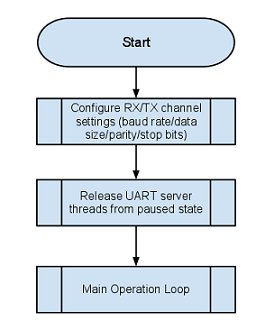
\includegraphics[width=0.500\linewidth]{muart_config_flow.png}
\end{sidecaption}\end{figure} \DocumentFooterFix



% NON-FULLWIDTH SECTION
\subsection{Webserver}
\label{programming_guide:webserver}

The webserver handles all HTTP requests from the web clients. A web client may request to change UART settings, save current settings, or apply the previously saved UART seetings etc. Webserver identifies these requests, validates them and services those requests. It calls appropriate UART handler api's to retrieve and set channel settings. For example, for a `Set' request from the web page, the webserver handler utilizes website component in order to parse the form data from web page, the required UART parameters are extracted and the UART\_Handler's uart\_set\_config api is called to set the new UART configuration.


The Webserver interface utilises \emph{sc\_website} component to implement web server functionality. Refer to the \emph{Quickstart Guide} within \emph{Documentation} or \emph{Developer Column} of the \verb`Slicekit GPIO and Ethernet Combo Demo` example in xSOFTip browser. This documentation contains more information on how to utilize the \verb`Embedded Webserver Function Library` component in customizing web server applications.



% NON-FULLWIDTH SECTION
\subsection{Flash interface}
\label{programming_guide:flash-interface}\begin{description}
\item[The s2e\_flash core handles data to/from flash fitted on board. The UART configuration web (html) pages, UART settings and IP configuration are typically stored into flash. Web pages are retrieved upon request from the client to the web server. UART settings can be `saved' and `restored' from flash. They are usually done via:]\begin{itemize}
\item   Request from web page (HTTP request)

\item   From Telnet configuration server

\item   Upon startup (to restore restore last saved settings)

\end{itemize}


\end{description}



IP configuration is saved via UDP server request and is requested from flash upon start-up.



% FULLWIDTH SECTION (with summary)
\clearpage
\chapter{API}
\label{api:api}\label{api::doc}\label{api:sec-api}%summary!
\begin{inthisdocument}
\item \nameref{api:configuration-defines}
\item \nameref{api:sec-const}
\item \nameref{api:data-structures}
\item \nameref{api:sec-conf-func}
\item \nameref{api:sec-xface-func}
\item \nameref{api:sec-module-func}
\end{inthisdocument}

\begin{fullwidth} % chapter!


\section{Configuration defines}
\label{api:configuration-defines}\label{api:sec-conf-defines}

The files multi\_uart\_tx\_conf.h and multi\_uart\_rx\_conf.h must be copied from
app\_multi\_uart\_demo\textbackslash{}src folder to app\_serial\_to\_ethernet\_demo\textbackslash{}src folder


\textbf{UART\_RX\_CHAN\_COUNT}
\begin{indentation}{\forceindentlen}{0mm}

Default value = 8


Define the number of channels that are to be supported, must fit in the port. Also, must be a power of 2 (i.e. 1,2,4,8) - not all channels have to be utilised
\end{indentation}

\textbf{UART\_TX\_CHAN\_COUNT}
\begin{indentation}{\forceindentlen}{0mm}

Default value = 8


Define the number of channels that are to be supported, must fit in the port. Also, must be a power of 2 (i.e. 1,2,4,8) - not all channels have to be utilised
\end{indentation}

\textbf{UART\_RX\_MAX\_BAUD}
\begin{indentation}{\forceindentlen}{0mm}

Default value = 115200


Define maximum baud rate to be supprted for any of the UART channel
\end{indentation}

\textbf{UART\_TX\_BUF\_SIZE}
\begin{indentation}{\forceindentlen}{0mm}

Default value = 8


Define the buffer size in UART word entries - needs to be a power of 2 (i.e. 1,2,4,8,16,32 etc)
\end{indentation}

The file xtcp\_client\_conf.h defines configuration fexibility required for XTCP clients in order to use XTCP server functions


\textbf{UIP\_CONF\_RECEIVE\_WINDOW}
\begin{indentation}{\forceindentlen}{0mm}

Default value = 128


Define window length of TCP packets that the application will receive and process for each TCP packets received from XTCP clients.
Note this value will be set as default length of application buffers that will be used to hold UART data collected from XTCP clients.
\end{indentation}

\textbf{XTCP\_CLIENT\_BUF\_SIZE}
\begin{indentation}{\forceindentlen}{0mm}

Default value = 650


Define MTU size used for XTCP device packet transmissions
\end{indentation}

The file udp\_discovery.h defines ports used for UDP discovery.
This file can set the following defines:


\textbf{UDP\_RECV\_BUF\_SIZE}
\begin{indentation}{\forceindentlen}{0mm}

Default value = 80


Define length of UDP message buffer which holds the incoming UDP test server request
or its corresponding S2E response
\end{indentation}

\textbf{INCOMING\_UDP\_PORT}
\begin{indentation}{\forceindentlen}{0mm}

Default value = 15534


Define incoming UDP port to listen to device discovery requests from UDP test server
\end{indentation}

\textbf{OUTGOING\_UDP\_PORT}
\begin{indentation}{\forceindentlen}{0mm}

Default value = 15533


Define outgoing UDP port in order to send device response to UDP test server
\end{indentation}

\textbf{S2E\_FIRMWARE\_VER}
\begin{indentation}{\forceindentlen}{0mm}

Current value = 1.1.2


Define to specify S2E firmware version. This shall be updated for every release
\end{indentation}

\textbf{UART\_RX\_FLUSH\_DELAY}
\begin{indentation}{\forceindentlen}{0mm}

Default value = 20000000


If UART data received is lesser than minimum configured packet size, this defines a
minimum wait time to send this data to telnet handler
\end{indentation}

The file telnet\_config.h defines ports used for Telnet socket used for UART configuration.


\textbf{S2E\_TELNET\_CONFIG\_PORT}
\begin{indentation}{\forceindentlen}{0mm}

Default value = 23


Define to specify telnet port to use for UART configuration
\end{indentation}

\section{Constants}
\label{api:sec-const}\label{api:constants}

The file srcs2e\_flash.h has some constants defined which may be used by other files while accessing flash.


\textbf{S2E\_FLASH\_ERROR}
\begin{indentation}{\forceindentlen}{0mm}

Default value = -1


Any errors (like flash not present, wrong flash, unable to write, etc...) while accessing the flash fitted on the board, are represented using this constant.
\end{indentation}

\textbf{S2E\_FLASH\_OK}
\begin{indentation}{\forceindentlen}{0mm}

Default value = 0


All successfull flash operations are represented using this constant.
\end{indentation}

\textbf{UART\_CONFIG}
\begin{indentation}{\forceindentlen}{0mm}

Default value = 0


To be used as a data type parameter while calling flash routines. This also represents the sector index (relative to webpage image) in the flash where UART configuration must be stored.
\end{indentation}

\textbf{IPVER}
\begin{indentation}{\forceindentlen}{0mm}

Default value = 1


To be used as a data type parameter while calling flash routines. This also represents the sector index (relative to webpage image) in the flash where IP configuration must be stored.
\end{indentation}

\textbf{FLASH\_CMD\_SAVE}
\begin{indentation}{\forceindentlen}{0mm}

Default value = 1


Flash command to `save' configuration to flash.
\end{indentation}

\textbf{FLASH\_CMD\_RESTORE}
\begin{indentation}{\forceindentlen}{0mm}

Default value = 2


Flash command to `restore' configuration from flash.
\end{indentation}

\textbf{FLASH\_DATA\_PRESENT}
\begin{indentation}{\forceindentlen}{0mm}

Default value = \$


While `saving' settings to flash, this value is written as the first byte. So, on a `restore' command, by reading for this sybol, we would know that some data is present in that sector of flash.
\end{indentation}

\section{Data structures}
\label{api:data-structures}\label{api:sec-data-struct}\index{uart\_config\_data\_t (C type)}

\textbf{\large uart\_config\_data\_t}


\vspace{2mm}

%before save

\begin{indentation*}{\apilargeindentlen}{0mm}%\vspace{-2mm}
\sloppy %%


Structure to hold UART configuration details.




\vspace{0.5\baselineskip}
\textbf{Fields}

\begin{apilist}[topsep=0pt]

\addtolength{\codeindent}{22mm}\index{uart\_config\_data\_t.channel\_id (C member)}\phantomsection\label{api:uart_config_data_t.channel_id}\item[int channel\_id]

UART Id.
\index{uart\_config\_data\_t.parity (C member)}\phantomsection\label{api:uart_config_data_t.parity}\item[e\_uart\_config\_parity parity]

One of valid parity: Odd, Even, Mark, Space, None.
\index{uart\_config\_data\_t.stop\_bits (C member)}\phantomsection\label{api:uart_config_data_t.stop_bits}\item[e\_uart\_config\_stop\_bits stop\_bits]

Stop bits configuration: Single or Two.
\index{uart\_config\_data\_t.polarity (C member)}\phantomsection\label{api:uart_config_data_t.polarity}\item[e\_uart\_config\_polarity polarity]

Polarity setting: Start bit as 1 or 0.
\index{uart\_config\_data\_t.baud (C member)}\phantomsection\label{api:uart_config_data_t.baud}\item[int baud]

Baud rate of UART channel.
\index{uart\_config\_data\_t.char\_len (C member)}\phantomsection\label{api:uart_config_data_t.char_len}\item[int char\_len]

Number of bits each UART character contain.
\addtolength{\codeindent}{-22mm}\end{apilist}


\end{indentation*}
\fussy


\section{Configuration functions}
\label{api:sec-conf-func}\label{api:configuration-functions}\index{uart\_config\_init (C function)}

\begin{minipage}{\linewidth}


\textbf{\large uart\_config\_init()}


\vspace{2mm}

%before save

\begin{indentation*}{\apilargeindentlen}{0mm}%\vspace{-2mm}
\sloppy %%


This function retrieves configuration of each UARTs from flash, and applies it to the base configuration structure of type uart\_config\_data\_t.


Telnet port applicable for corresponding UART is also fetched from flash and applied to repective UART configuration structure. If there is no valid flash configuration, default in-program configuration with following values EvenParity-1StopBit-115200Baud-Start0Polarity-8UARTCharLen is used




\vspace{0.5\baselineskip}


\textbf{Type}


\begin{indentation}{\apismallindentlen}{0mm}
\phantomsection\label{api:uart_config_init}

\texttt{\begin{nstabbing}void uart\_config\_init(\= chanend c\_uart\_config,\\ 
\> chanend ?c\_flash\_data,\\ 
\> chanend ?c\_xtcp,\\ 
\> int \&telnet\_port\_address)
\end{nstabbing}}


\end{indentation}



\textbf{Parameters}

\begin{indentation*}{\apismallindentlen}{0mm}%%


\begin{apilist}

\item[c\_uart\_config]Channel-end to communicate UART configuration details between TCP handler and UART handler thread
\item[c\_flash\_data]Channel-end to communicate UART configuration data stored in flash to TCP handler thread
\item[c\_xtcp]Channel-end between XTCP and TCP handler thread
\item[telnet\_port\_address]Reference to structure holding Telnet port addresses mapped for UARTs
\end{apilist}


\end{indentation*}




\textbf{Returns}

\begin{indentation*}{\apismallindentlen}{0mm}%%


None

\end{indentation*}

\end{indentation*}
\fussy


\end{minipage}
\index{s2e\_webserver\_init (C function)}

\begin{minipage}{\linewidth}


\textbf{\large s2e\_webserver\_init()}


\vspace{2mm}

%before save

\begin{indentation*}{\apilargeindentlen}{0mm}%\vspace{-2mm}
\sloppy %%


s2e\_webserver\_init The S2E webserver initialization routine.


Registers all channels used by it.




\vspace{0.5\baselineskip}


\textbf{Type}


\begin{indentation}{\apismallindentlen}{0mm}
\phantomsection\label{api:s2e_webserver_init}

\texttt{\begin{nstabbing}void s2e\_webserver\_init(\= chanend c\_xtcp,\\ 
\> chanend ?c\_flash,\\ 
\> chanend c\_uart\_config,\\ 
\> chanend ?c\_flash\_data)
\end{nstabbing}}


\end{indentation}



\textbf{Parameters}

\begin{indentation*}{\apismallindentlen}{0mm}%%


\begin{apilist}

\item[c\_xtcp]channel connecting to the xtcp module
\item[c\_flash]channel for web page data
\item[c\_uart\_config]channel for UART configuration
\item[c\_flash\_data]channel for s2e flash data
\end{apilist}


\end{indentation*}




\textbf{Returns}

\begin{indentation*}{\apismallindentlen}{0mm}%%


none

\end{indentation*}

\end{indentation*}
\fussy


\end{minipage}
\index{telnet\_to\_uart\_init (C function)}

\begin{minipage}{\linewidth}


\textbf{\large telnet\_to\_uart\_init()}


\vspace{2mm}

%before save

\begin{indentation*}{\apilargeindentlen}{0mm}%\vspace{-2mm}
\sloppy %%


This function initializes UART state structure, assigns configured/default telnet ports and listens on these ports, shares UART buffer references to UART handler thread.




\vspace{0.5\baselineskip}


\textbf{Type}


\begin{indentation}{\apismallindentlen}{0mm}
\phantomsection\label{api:telnet_to_uart_init}

\texttt{\begin{nstabbing}void telnet\_to\_uart\_init(\= chanend c\_xtcp,\\ 
\> chanend c\_uart\_data,\\ 
\> int telnet\_port\_address{[}{]})
\end{nstabbing}}


\end{indentation}



\textbf{Parameters}

\begin{indentation*}{\apismallindentlen}{0mm}%%


\begin{apilist}

\item[c\_xtcp]Channel-end between XTCP and TCP handler thread
\item[c\_uart\_data]Channel-end to communicate UART data between TCP handler and UART handler thread
\item[telnet\_port\_address]Array contining telnet ports mapped for configured UARTs
\end{apilist}


\end{indentation*}




\textbf{Returns}

\begin{indentation*}{\apismallindentlen}{0mm}%%


None

\end{indentation*}

\end{indentation*}
\fussy


\end{minipage}
\index{udp\_discovery\_init (C function)}

\begin{minipage}{\linewidth}


\textbf{\large udp\_discovery\_init()}


\vspace{2mm}

%before save

\begin{indentation*}{\apilargeindentlen}{0mm}%\vspace{-2mm}
\sloppy %%


This function initializes UDP discovery state, fetches S2E IP address stored in flash and references to ETH thread in order to configure device IP.


If valid IP is not present in flash, default configured IP defined from ipconfig is used




\vspace{0.5\baselineskip}


\textbf{Type}


\begin{indentation}{\apismallindentlen}{0mm}
\phantomsection\label{api:udp_discovery_init}

\texttt{\begin{nstabbing}void udp\_discovery\_init(\= chanend c\_xtcp,\\ 
\> chanend c\_flash\_data,\\ 
\> xtcp\_ipconfig\_t \&ipconfig)
\end{nstabbing}}


\end{indentation}



\textbf{Parameters}

\begin{indentation*}{\apismallindentlen}{0mm}%%


\begin{apilist}

\item[c\_xtcp]Channel between XTCP and TCP handler thread
\item[c\_flash\_data]Channel between Flash and TCP handler thread
\item[ipconfig]Reference to structure holding IP configuration info
\end{apilist}


\end{indentation*}




\textbf{Returns}

\begin{indentation*}{\apismallindentlen}{0mm}%%


None

\end{indentation*}

\end{indentation*}
\fussy


\end{minipage}


\section{Interface functions}
\label{api:}\label{api:sec-xface-func}\label{api:interface-functions}\index{uart\_handler (C function)}

\begin{minipage}{\linewidth}


\textbf{\large uart\_handler()}


\vspace{2mm}

%before save

\begin{indentation*}{\apilargeindentlen}{0mm}%\vspace{-2mm}
\sloppy %%


This function configures UARTs, initializes application buffers states.


As a part of event handling, this function does the following: (i) handles incoming data from UARTs and stores into appropirate buffers (ii) in case of data transfer transaction, either notifies or acknowledges TCP handler about UART data; otherwise, listens from TCP handler to (a) collect telnet received data to UART (b) share appropriate UART buffer holding UART recived data (iii) in case of UART configuration requests, collects appropriate UART configuration and reconfigures UART for received configuration (iv) sends a data byte from telnet UART buffers in a round robin basis, and notifies current transmit and receive transactions




\vspace{0.5\baselineskip}


\textbf{Type}


\begin{indentation}{\apismallindentlen}{0mm}
\phantomsection\label{api:uart_handler}

\texttt{\begin{nstabbing}void uart\_handler(\= chanend c\_uart\_data,\\ 
\> chanend c\_uart\_config,\\ 
\> streaming chanend c\_uart\_rx,\\ 
\> streaming chanend c\_uart\_tx)
\end{nstabbing}}


\end{indentation}



\textbf{Parameters}

\begin{indentation*}{\apismallindentlen}{0mm}%%


\begin{apilist}

\item[c\_uart\_data]Channel-end to communicate UART data between TCP handler and UART handler thread
\item[c\_uart\_config]Channel-end to communicate UART configuration details between TCP handler and UART handler thread
\item[c\_uart\_rx]Channel primarily to send UART data from application to MultiUART RX server thread
\item[c\_uart\_tx]Channel primarily to collect UART data from MultiUART TX server thread into UART handler thread
\end{apilist}


\end{indentation*}




\textbf{Returns}

\begin{indentation*}{\apismallindentlen}{0mm}%%


None

\end{indentation*}

\end{indentation*}
\fussy


\end{minipage}
\index{tcp\_handler (C function)}

\begin{minipage}{\linewidth}


\textbf{\large tcp\_handler()}


\vspace{2mm}

%before save

\begin{indentation*}{\apilargeindentlen}{0mm}%\vspace{-2mm}
\sloppy %%


This function handles TCP handler thread.


During initialization, IP configuration details stored in flash are retrieved from UDP discovery function and passed on to ETH thread This thread mainly handles (a) all XTCP events and invokes respective sub-function handlers (b) notification messages from UART handler thread for UART data transactions




\vspace{0.5\baselineskip}


\textbf{Type}


\begin{indentation}{\apismallindentlen}{0mm}
\phantomsection\label{api:tcp_handler}

\texttt{\begin{nstabbing}void tcp\_handler(\= chanend c\_xtcp,\\ 
\> chanend c\_uart\_data,\\ 
\> chanend c\_uart\_config,\\ 
\> chanend ?c\_flash\_web,\\ 
\> chanend ?c\_flash\_data)
\end{nstabbing}}


\end{indentation}



\textbf{Parameters}

\begin{indentation*}{\apismallindentlen}{0mm}%%


\begin{apilist}

\item[c\_xtcp]Channel-end between XTCP and TCP handler thread
\item[c\_uart\_data]Channel-end to communicate UART data between TCP handler and UART handler thread
\item[c\_uart\_config]Channel-end to communicate UART configuration data TCP handler and UART handler thread
\item[c\_flash\_web]Channel-end to communicate Web page data stored in flash to TCP handler thread
\item[c\_flash\_data]Channel-end to communicate UART configuration data stored in flash to TCP handler thread
\end{apilist}


\end{indentation*}




\textbf{Returns}

\begin{indentation*}{\apismallindentlen}{0mm}%%


None

\end{indentation*}

\end{indentation*}
\fussy


\end{minipage}
\index{telnet\_config\_event\_handler (C function)}

\begin{minipage}{\linewidth}


\textbf{\large telnet\_config\_event\_handler()}


\vspace{2mm}

%before save

\begin{indentation*}{\apilargeindentlen}{0mm}%\vspace{-2mm}
\sloppy %%


This function handles UART configuration requests from telnet configuration client.


It initializes cofnig parse state machine, receives configuration request events, sends response back to the client




\vspace{0.5\baselineskip}


\textbf{Type}


\begin{indentation}{\apismallindentlen}{0mm}
\phantomsection\label{api:telnet_config_event_handler}

\texttt{\begin{nstabbing}void telnet\_config\_event\_handler(\= chanend c\_xtcp,\\ 
\> chanend c\_uart\_config,\\ 
\> chanend c\_flash\_data,\\ 
\> xtcp\_connection\_t \&conn)
\end{nstabbing}}


\end{indentation}



\textbf{Parameters}

\begin{indentation*}{\apismallindentlen}{0mm}%%


\begin{apilist}

\item[c\_xtcp]Channel-end between XTCP and TCP handler thread
\item[c\_uart\_configChannel-end]to communicate UART configuration data TCP handler and UART handler thread
\item[c\_flash\_data]Channel-end to communicate UART configuration data stored in flash to TCP handler thread
\item[conn]Reference to structure holding IP configuration info
\end{apilist}


\end{indentation*}




\textbf{Returns}

\begin{indentation*}{\apismallindentlen}{0mm}%%


None

\end{indentation*}

\end{indentation*}
\fussy


\end{minipage}
\index{s2e\_webserver\_event\_handler (C function)}

\begin{minipage}{\linewidth}


\textbf{\large s2e\_webserver\_event\_handler()}


\vspace{2mm}

%before save

\begin{indentation*}{\apilargeindentlen}{0mm}%\vspace{-2mm}
\sloppy %%


s2e\_webserver\_event\_handler Handles webserver event.




\vspace{0.5\baselineskip}


\textbf{Type}


\begin{indentation}{\apismallindentlen}{0mm}
\phantomsection\label{api:s2e_webserver_event_handler}

\texttt{\begin{nstabbing}void s2e\_webserver\_event\_handler(\= chanend c\_xtcp,\\ 
\> chanend ?c\_flash,\\ 
\> chanend c\_uart\_config,\\ 
\> xtcp\_connection\_t \&conn)
\end{nstabbing}}


\end{indentation}



\textbf{Parameters}

\begin{indentation*}{\apismallindentlen}{0mm}%%


\begin{apilist}

\item[c\_xtcp]channel connecting to the xtcp module
\item[c\_flash]channel for web page data
\item[c\_uart\_config]channel for UART configuration
\item[conn]XTCP connection state
\end{apilist}


\end{indentation*}




\textbf{Returns}

\begin{indentation*}{\apismallindentlen}{0mm}%%


none

\end{indentation*}

\end{indentation*}
\fussy


\end{minipage}
\index{telnet\_to\_uart\_event\_handler (C function)}

\begin{minipage}{\linewidth}


\textbf{\large telnet\_to\_uart\_event\_handler()}


\vspace{2mm}

%before save

\begin{indentation*}{\apilargeindentlen}{0mm}%\vspace{-2mm}
\sloppy %%


This function handles XTCP events related to Telnet data communication.


For any event, a correponding UART is mapped from XTCP connection As a part of event handling, this function does the following: (i) for new connections, TCP connection details are stored and telnet parse state machine and TCP ack mode is initialized (ii) for recieve events, data from TCP stack is collected into appropriate UART buffers. Received data is sent to telnet parser server in order to separate application data from telnet protocol. Initiates UART data transaction on c\_uart\_data channel in order to send data to UART (iii) for send requests initiated by telnet handler, this handler performs either of the following functionality (a) welcome messages are sent to respective telnet clients at the start of each session (b) collect outstanding data from appropriate UART RX active buffer and sends on XTCP connection




\vspace{0.5\baselineskip}


\textbf{Type}


\begin{indentation}{\apismallindentlen}{0mm}
\phantomsection\label{api:telnet_to_uart_event_handler}

\texttt{\begin{nstabbing}void telnet\_to\_uart\_event\_handler(\= chanend c\_xtcp,\\ 
\> chanend c\_uart\_data,\\ 
\> xtcp\_connection\_t \&conn)
\end{nstabbing}}


\end{indentation}



\textbf{Parameters}

\begin{indentation*}{\apismallindentlen}{0mm}%%


\begin{apilist}

\item[c\_xtcp]Channel-end between XTCP and TCP handler thread
\item[c\_uart\_data]Channel-end to communicate UART data between TCP handler and UART handler thread
\item[conn]Reference to structure holding IP configuration info
\end{apilist}


\end{indentation*}




\textbf{Returns}

\begin{indentation*}{\apismallindentlen}{0mm}%%


None

\end{indentation*}

\end{indentation*}
\fussy


\end{minipage}
\index{udp\_discovery\_event\_handler (C function)}

\begin{minipage}{\linewidth}


\textbf{\large udp\_discovery\_event\_handler()}


\vspace{2mm}

%before save

\begin{indentation*}{\apilargeindentlen}{0mm}%\vspace{-2mm}
\sloppy %%


Handles events related to UDP discovery functionality.


Receives S2E identification and IP configuration requests from UDP test server, frames and sends S2E response messages




\vspace{0.5\baselineskip}


\textbf{Type}


\begin{indentation}{\apismallindentlen}{0mm}
\phantomsection\label{api:udp_discovery_event_handler}

\texttt{\begin{nstabbing}void udp\_discovery\_event\_handler(\= chanend c\_xtcp,\\ 
\> chanend c\_flash\_data,\\ 
\> xtcp\_connection\_t \&conn)
\end{nstabbing}}


\end{indentation}



\textbf{Parameters}

\begin{indentation*}{\apismallindentlen}{0mm}%%


\begin{apilist}

\item[c\_xtcp]Channel between XTCP and TCP handler thread
\item[c\_flash\_data]Channel between Flash and TCP handler thread
\item[conn]Reference to UDP connection state
\end{apilist}


\end{indentation*}




\textbf{Returns}

\begin{indentation*}{\apismallindentlen}{0mm}%%


None

\end{indentation*}

\end{indentation*}
\fussy


\end{minipage}
\index{s2e\_flash (C function)}

\begin{minipage}{\linewidth}


\textbf{\large s2e\_flash()}


\vspace{2mm}

%before save

\begin{indentation*}{\apilargeindentlen}{0mm}%\vspace{-2mm}
\sloppy %%


s2e\_flash The S2E flash thread will keep looking for data (or commands) on the c\_flash\_data channel.




\vspace{0.5\baselineskip}


\textbf{Type}


\begin{indentation}{\apismallindentlen}{0mm}
\phantomsection\label{api:s2e_flash}

\texttt{\begin{nstabbing}void s2e\_flash(\= chanend c\_flash\_web,\\ 
\> chanend c\_flash\_data,\\ 
\> fl\_SPIPorts \&flash\_ports)
\end{nstabbing}}


\end{indentation}



\textbf{Parameters}

\begin{indentation*}{\apismallindentlen}{0mm}%%


\begin{apilist}

\item[c\_flash\_web]channel for webpage data
\item[c\_flash\_data]channel for s2e data
\item[flash\_ports]reference to flash ports used by the device
\end{apilist}


\end{indentation*}




\textbf{Returns}

\begin{indentation*}{\apismallindentlen}{0mm}%%


none

\end{indentation*}

\end{indentation*}
\fussy


\end{minipage}
\index{send\_data\_to\_flash\_thread (C function)}

\begin{minipage}{\linewidth}


\textbf{\large send\_data\_to\_flash\_thread()}


\vspace{2mm}

%before save

\begin{indentation*}{\apilargeindentlen}{0mm}%\vspace{-2mm}
\sloppy %%


send\_data\_to\_flash\_thread Send UART configuration data to flash.


Send one configuration at a time. In order to send configuration for all the channels, this routine must be called in a loop; each time sending the current channels config.




\vspace{0.5\baselineskip}


\textbf{Type}


\begin{indentation}{\apismallindentlen}{0mm}
\phantomsection\label{api:send_data_to_flash_thread}

\texttt{\begin{nstabbing}void send\_data\_to\_flash\_thread(\= chanend c\_flash\_data,\\ 
\> {\hyperref[api:uart_config_data_t]{uart\_config\_data\_t}} \&data)
\end{nstabbing}}


\end{indentation}



\textbf{Parameters}

\begin{indentation*}{\apismallindentlen}{0mm}%%


\begin{apilist}

\item[c\_flash\_data]channel for s2e data
\item[data]reference to the current channel's config
\end{apilist}


\end{indentation*}




\textbf{Returns}

\begin{indentation*}{\apismallindentlen}{0mm}%%


none

\end{indentation*}

\end{indentation*}
\fussy


\end{minipage}
\index{get\_data\_from\_flash\_thread (C function)}

\begin{minipage}{\linewidth}


\textbf{\large get\_data\_from\_flash\_thread()}


\vspace{2mm}

%before save

\begin{indentation*}{\apilargeindentlen}{0mm}%\vspace{-2mm}
\sloppy %%


get\_data\_from\_flash\_thread Get UART configuration data from flash.


Get one configuration at a time. In order to get configuration for all the channels, this routine must be called in a loop; each time updating the current channels config. Telnet ports for each channel are also updated.




\vspace{0.5\baselineskip}


\textbf{Type}


\begin{indentation}{\apismallindentlen}{0mm}
\phantomsection\label{api:get_data_from_flash_thread}

\texttt{\begin{nstabbing}void get\_data\_from\_flash\_thread(\= chanend c\_flash\_data,\\ 
\> {\hyperref[api:uart_config_data_t]{uart\_config\_data\_t}} \&data,\\ 
\> int \&telnet\_port)
\end{nstabbing}}


\end{indentation}



\textbf{Parameters}

\begin{indentation*}{\apismallindentlen}{0mm}%%


\begin{apilist}

\item[c\_flash\_data]channel for s2e data
\item[data]reference to the current channel's config to update
\item[telnet\_port]reference to current channel's telnet port to update
\end{apilist}


\end{indentation*}




\textbf{Returns}

\begin{indentation*}{\apismallindentlen}{0mm}%%


none

\end{indentation*}

\end{indentation*}
\fussy


\end{minipage}
\index{send\_ipconfig\_to\_flash\_thread (C function)}

\begin{minipage}{\linewidth}


\textbf{\large send\_ipconfig\_to\_flash\_thread()}


\vspace{2mm}

%before save

\begin{indentation*}{\apilargeindentlen}{0mm}%\vspace{-2mm}
\sloppy %%


send\_ipconfig\_to\_flash\_thread Send IP configuration data to flash.




\vspace{0.5\baselineskip}


\textbf{Type}


\begin{indentation}{\apismallindentlen}{0mm}
\phantomsection\label{api:send_ipconfig_to_flash_thread}

\texttt{\begin{nstabbing}void send\_ipconfig\_to\_flash\_thread(\= chanend c\_flash\_data,\\ 
\> xtcp\_ipconfig\_t \&ip)
\end{nstabbing}}


\end{indentation}



\textbf{Parameters}

\begin{indentation*}{\apismallindentlen}{0mm}%%


\begin{apilist}

\item[c\_flash\_data]channel for s2e data
\item[ip]reference to the current IP config
\end{apilist}


\end{indentation*}




\textbf{Returns}

\begin{indentation*}{\apismallindentlen}{0mm}%%


none

\end{indentation*}

\end{indentation*}
\fussy


\end{minipage}
\index{get\_ipconfig\_from\_flash\_thread (C function)}

\begin{minipage}{\linewidth}


\textbf{\large get\_ipconfig\_from\_flash\_thread()}


\vspace{2mm}

%before save

\begin{indentation*}{\apilargeindentlen}{0mm}%\vspace{-2mm}
\sloppy %%


get\_ipconfig\_from\_flash\_thread Get IP configuration data from flash.




\vspace{0.5\baselineskip}


\textbf{Type}


\begin{indentation}{\apismallindentlen}{0mm}
\phantomsection\label{api:get_ipconfig_from_flash_thread}

\texttt{\begin{nstabbing}void get\_ipconfig\_from\_flash\_thread(\= chanend c\_flash\_data,\\ 
\> xtcp\_ipconfig\_t \&ip)
\end{nstabbing}}


\end{indentation}



\textbf{Parameters}

\begin{indentation*}{\apismallindentlen}{0mm}%%


\begin{apilist}

\item[c\_flash\_data]channel for s2e data
\item[ip]reference to the current IP config
\end{apilist}


\end{indentation*}




\textbf{Returns}

\begin{indentation*}{\apismallindentlen}{0mm}%%


none

\end{indentation*}

\end{indentation*}
\fussy


\end{minipage}
\index{send\_cmd\_to\_flash\_thread (C function)}

\begin{minipage}{\linewidth}


\textbf{\large send\_cmd\_to\_flash\_thread()}


\vspace{2mm}

%before save

\begin{indentation*}{\apilargeindentlen}{0mm}%\vspace{-2mm}
\sloppy %%


send\_cmd\_to\_flash\_thread Send command to flash thread.




\vspace{0.5\baselineskip}


\textbf{Type}


\begin{indentation}{\apismallindentlen}{0mm}
\phantomsection\label{api:send_cmd_to_flash_thread}

\texttt{\begin{nstabbing}void send\_cmd\_to\_flash\_thread(\= chanend c\_flash\_data,\\ 
\> int data\_type,\\ 
\> int command)
\end{nstabbing}}


\end{indentation}



\textbf{Parameters}

\begin{indentation*}{\apismallindentlen}{0mm}%%


\begin{apilist}

\item[c\_flash\_data]channel for s2e data
\item[data\_type]UART\_CONFIG (or) IPVER
\item[command]FLASH\_CMD\_SAVE (or) FLASH\_CMD\_RESTORE
\end{apilist}


\end{indentation*}




\textbf{Returns}

\begin{indentation*}{\apismallindentlen}{0mm}%%


none

\end{indentation*}

\end{indentation*}
\fussy


\end{minipage}
\index{get\_flash\_access\_result (C function)}

\begin{minipage}{\linewidth}


\textbf{\large get\_flash\_access\_result()}


\vspace{2mm}

%before save

\begin{indentation*}{\apilargeindentlen}{0mm}%\vspace{-2mm}
\sloppy %%


get\_flash\_access\_result Get the flash access result after performing certain command.




\vspace{0.5\baselineskip}


\textbf{Type}


\begin{indentation}{\apismallindentlen}{0mm}
\phantomsection\label{api:get_flash_access_result}

\texttt{\begin{nstabbing}int get\_flash\_access\_result(chanend c\_flash\_data)
\end{nstabbing}}


\end{indentation}



\textbf{Parameters}

\begin{indentation*}{\apismallindentlen}{0mm}%%


\begin{apilist}

\item[c\_flash\_data]channel for s2e data
\end{apilist}


\end{indentation*}




\textbf{Returns}

\begin{indentation*}{\apismallindentlen}{0mm}%%


int S2E\_FLASH\_ERROR (or) S2E\_FLASH\_OK

\end{indentation*}

\end{indentation*}
\fussy


\end{minipage}


\section{Module functions}
\label{api:}\label{api:sec-module-func}\label{api:module-functions}\index{parse\_telnet\_buffer (C function)}

\begin{minipage}{\linewidth}


\textbf{\large parse\_telnet\_buffer()}


\vspace{2mm}

%before save

\begin{indentation*}{\apilargeindentlen}{0mm}%\vspace{-2mm}
\sloppy %%


This function implements Telnet server functionality.


Mainly extracts application data from XTCP data packets in telnet protocol format.




\vspace{0.5\baselineskip}


\textbf{Type}


\begin{indentation}{\apismallindentlen}{0mm}
\phantomsection\label{api:parse_telnet_buffer}

\texttt{\begin{nstabbing}int parse\_telnet\_buffer(\= char data{[}{]},\\ 
\> int len,\\ 
\> int \&parse\_state,\\ 
\> int \&close\_request)
\end{nstabbing}}


\end{indentation}



\textbf{Parameters}

\begin{indentation*}{\apismallindentlen}{0mm}%%


\begin{apilist}

\item[data]Buffer to store application data filtered from telnet server
\item[len]Number of bytes of received data
\item[parse\_state]Current state of telnet parser state machine
\item[close\_request]Flag to set when telnet client is suspended
\end{apilist}


\end{indentation*}




\textbf{Returns}

\begin{indentation*}{\apismallindentlen}{0mm}%%


Length of application buffer

\end{indentation*}

\end{indentation*}
\fussy


\end{minipage}
\end{fullwidth}%


% NON-FULLWIDTH SECTION
\clearpage
\chapter{Using the application}
\label{using_the_application:}\label{using_the_application::doc}\label{using_the_application:using-the-application}%summary!
\begin{inthisdocument}
\item \nameref{using_the_application:s2e-device-discovery}
\item \nameref{using_the_application:data-communication-using-s2e-device}
\item \nameref{using_the_application:device-configuration-using-web-interface}
\item \nameref{using_the_application:device-configuration-using-telnet-interface}
\end{inthisdocument}



This section details on how to use the application and its user interfaces.



% NON-FULLWIDTH SECTION
\section{S2E device discovery}
\label{using_the_application:s2e-device-discovery}

S2E devices discovery on the network is performed by a UDP test server script (available at \verb`sw_serial_to_ethernet -> tests -> udp_test_server`).
This script needs to be executed on a host machine connected to a network router.
\begin{itemize}
\item   Make sure the device is flashed with the firmware and web pages

\item   For Windows users, download \emph{Serial\_to\_Ethernet\_UDP\_test\_server} package (XM-004697-SM) and extract its contents to a directory. Navigate to (udp\_test\_server -\textgreater{} windows -\textgreater{} udp\_server.exe), right-click on udp-server.exe and run as Administrator.

\item   For MAC or Linux users, it is recommended to install socket package for python, and run the script using the command \emph{python udp\_server.py}

\end{itemize}




% NON-FULLWIDTH SECTION
\subsection{Running the UDP test server}
\label{using_the_application:running-the-udp-test-server}\begin{enumerate}
\item   Select an appropriate host specific option as described above

\item   Script displays the selected network adapter on the console. If there are multiple network adapters on your host, ensure the ip address used by the script corresponds to the one used by your network adapter connected to the router

\item   Script displays different options to choose as explained in the following sections:

\end{enumerate}

\begin{figure}[h]
\begin{sidecaption}{S2E device discovery using udp\_test\_server}

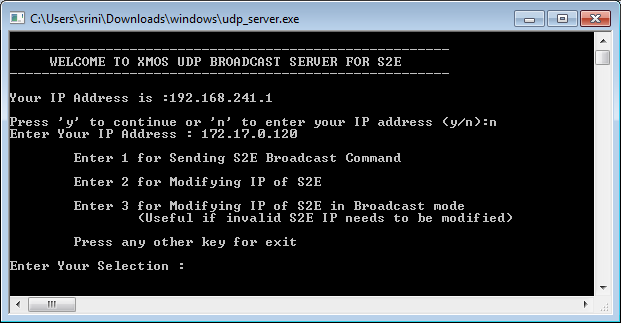
\includegraphics[width=0.500\linewidth]{udp_test_server.png}
\end{sidecaption}\end{figure} \DocumentFooterFix



% NON-FULLWIDTH SECTION
\subsection{Discover the S2E devices on the network}
\label{using_the_application:discover-the-s2e-devices-on-the-network}\begin{enumerate}
\item   Key in option \emph{1} from the choices.

\item   Once the script is executed, it sends a broadcast request for all S2E devices in the network to respond.
The message format is ``XMOS S2E REPLY'' broadcasted to 255.255.255.255

\item   XMOS S2E devices monitor this broadcast message and responds to the test server using the following format:
``XMOS S2E VER:a.b.c;MAC:xx:xx:xx:xx:xx:xx;IP:abc.def.uvw.xyz''

\item   The test server parses this response received from S2E devices available in the network and displays
the following information on the console:
VER --\textgreater{} Firmware Version
MAC --\textgreater{} MAC Address
IP --\textgreater{} IP address of the S2E device

\item   The above information is displayed for all the S2E devices available in the network

\end{enumerate}




% NON-FULLWIDTH SECTION
\subsection{Modify IP address of a particular S2E device}
\label{using_the_application:modify-ip-address-of-a-particular-s2e-device}\begin{enumerate}
\item   Key in option \emph{2} from the choices.

\item   The device discovery (option 1) should be used prior to using this option

\item   Upon selecting the above option, ensure all available S2Es on the network are displayed

\item   You can now select an appropriate S2E from the list and provide a new IP address for the selected S2E device.
The server sends a unicast message using the format: ``XMOS S2E IPCHANGE aaa.bbb.ccc.ddd''

\item   Appropriate S2E device will receive this message, flash the new ip address, resets and starts with the new ip address

\item   At the test server, you can now see S2E IP is changed to the new IP address by selecting the device discovery option again

\end{enumerate}




% NON-FULLWIDTH SECTION
\subsection{Modify IP address of all S2E devices to use DHCP server}
\label{using_the_application:modify-ip-address-of-all-s2e-devices-to-use-dhcp-server}\begin{enumerate}
\item   Key in option \emph{3} from the choices.

\item   This is a request and enables the s2e devices to DHCP mode. A DHCP server can be used to assign IP address to all S2E devices.
The test server sends a broadcast message using the format: ``XMOS S2E IPCHANGE 0.0.0.0''

\item   It is important that only the intended S2Es for which the IP address is invalid should be made available in the network
All other S2Es should be removed from the network.

\item   Once the S2E devices IP is changed to the DHCP assigned IP addresses, select discovery option after some time in order to know the the new IP addresses for the device(s)

\end{enumerate}




% NON-FULLWIDTH SECTION
\section{Data communication using S2E device}
\label{using_the_application:data-communication-using-s2e-device}

Apart from the standard UART and Telnet clients available on the host, following tools may be installed on the host system in order to use the S2E application.
\begin{itemize}
\item   For Win 7 users, Hercules Utility by HW-Group available at \parurl{http://www.hw-group.com/products/hercules/index\_en.html}

\item   For MAC users, SecureCRT7.0 utility available at \parurl{http://www.vandyke.com/download/securecrt/}

\end{itemize}



The following example uses Hercules 3.2.5



% NON-FULLWIDTH SECTION
\subsection{UART serial port setup}
\label{using_the_application:uart-serial-port-setup}\begin{enumerate}
\item   Open the client application and change to \verb`Serial` tab

\item   Select appropriate options in the \verb`Serial` pane.
Apply the default settings (Data size = 8, Parity = Even, Handshake = Off, Mode = Free)
Cross check these settings with the UART settings in the webpage.

\item   Click \verb`Open`

\end{enumerate}




% NON-FULLWIDTH SECTION
\subsection{Telnet client setup}
\label{using_the_application:telnet-client-setup}\begin{enumerate}
\item   Open the client application

\item   Switch to \verb`TCP Client` tab

\item   Key in the ip address (for e.g. 169.254.196.178) of the s2e device

\item   Key in the port number configured for a particular UART (default configured values for each uart channel starts with 46)

\item   Click \verb`Connect`

\end{enumerate}



Telnet client connection to the s2e server is now opened; now key in the data to be sent to a particular UART.
Files can also be uploaded using this client by right-clicking (and selecting appropriate option) in the \verb`data` pane of either sessions.


Software is tested for the following telnet clients
\begin{enumerate}
\item   Putty

\item   Hercules

\end{enumerate}




% NON-FULLWIDTH SECTION
\section{Device configuration using web interface}
\label{using_the_application:device-configuration-using-web-interface}\begin{enumerate}
\item   Open the browser window

\item   Key in the ip address (for e.g. \xurl{http://169.254.196.178/}) of the S2E device and press \verb`Enter`.

\end{enumerate}



Home page of the application appears
\begin{enumerate}
\item   Click on a \verb`UART Channel` to configure.

\end{enumerate}



A new page for the selected channel appears with its settings. In order to change the UART parameters
\begin{enumerate}
\item   Select UART parameters to change (Parity, Stop bits, Baud rate, Char Len or Telnet port)

\item   Click \verb`Set`.

\item   If configuration is set successfully, the \verb`Response` text will say `Ok'

\item   Click on \verb`Back to main config page` to select a different UART channel or save the current settings to flash.

\item   When clicked on \verb`Save` in the main config page, current set configuration will be saved to flash. On successfull save, the \verb`Response` text will say `Ok'

\end{enumerate}



Software is tested for the following web browsers
\begin{enumerate}
\item   Google Chrome

\item   Mozilla Firefox

\end{enumerate}




% NON-FULLWIDTH SECTION
\section{Device configuration using telnet interface}
\label{using_the_application:device-configuration-using-telnet-interface}

Telnet client can also be used for UART configuration or passing client data to UART channels (and vice versa). These are described as follows:



% NON-FULLWIDTH SECTION
\subsection{UART configuration}
\label{using_the_application:uart-configuration}

A separate telnet socket (default configured to port 23) is used for configuring UART channels via telnet client.
\begin{enumerate}
\item   Open the telnet client (following example uses Hercules 3.2.5)

\item   Switch to \verb`TCP Client` tab

\item   Key in the ip address (for e.g. 169.254.196.178)

\item   Key in the port number (for UART config, it is 23)

\item   Click \verb`Connect`

\end{enumerate}



UART configuration server's welcome message appears in the data pane of Telnet client


Use the following format for configuring an UART channel
\textasciitilde{}C\textasciitilde{}\textasciitilde{}P1\textasciitilde{}\textasciitilde{}P2\textasciitilde{}\textasciitilde{}P3\textasciitilde{}\textasciitilde{}P4\textasciitilde{}\textasciitilde{}P5\textasciitilde{}\textasciitilde{}P6\textasciitilde{}@
\begin{itemize}
\item   \textasciitilde{} is the parameter separator

\item   @ is command termination marker

\item   \begin{description}
\item[C]{[}Command code{]}

1 : Get channel configuration for a particular channel
2 : Set channel configuration
3 : Save current configuration of all channels to flash
4 : Restore and set channel configuration from flash

\end{description}


\item   P1 : UART Channel Identifier (typical values range for 0 to 7)

\item   \begin{description}
\item[P2]{[}Parity Configuration (typical values range for 0 to 4){]}

0 : No Parity
1 : Odd Parity
2 : Even Parity
3 : Mark (always 1) parity bit
4 : Space (always 0) parity bit

\end{description}


\item   \begin{description}
\item[P3]{[}Stop bits configuration (typical values are 0 or 1){]}

0 : Single stop bit
1 : Two stop bits

\end{description}


\item   \begin{description}
\item[P4]{[}Baud rate configuration. Typical values (bits per second) include{]}

115200
57600
38400
28800
19200
14400
9600
7200
4800
2400
1200
600
300
150

\end{description}


\item   \begin{description}
\item[P5]{[}UART character length. Typical values include{]}

5
6
7
8
9

\end{description}


\item   P6 : Telnet port (typical values are 10 to 65536)

\end{itemize}

\begin{enumerate}
\item   Click \verb`Enter` to apply the configuration for the channel

\end{enumerate}




% NON-FULLWIDTH SECTION
\subsection{Sample usage}
\label{using_the_application:sample-usage}\begin{itemize}
\item   \begin{description}
\item[Get: \textasciitilde{}1\textasciitilde{}\textasciitilde{}0\textasciitilde{}@]

Gets channel `0' configuration.

\end{description}


\item   \begin{description}
\item[Set: \textasciitilde{}2\textasciitilde{}\textasciitilde{}0\textasciitilde{}\textasciitilde{}2\textasciitilde{}\textasciitilde{}0\textasciitilde{}\textasciitilde{}115200\textasciitilde{}\textasciitilde{}8\textasciitilde{}\textasciitilde{}100\textasciitilde{}@]

Sets channel `0' with: Even parity, single stop bits, 115200 baud, 8 character length and telnet port to communicate with this channel as 100.

\end{description}


\item   \begin{description}
\item[Save: \textasciitilde{}3\textasciitilde{}@]

Save current set configuration of all channels to flash

\end{description}


\item   \begin{description}
\item[Restore: \textasciitilde{}4\textasciitilde{}@]

Restores and sets channels configuration from flash

\end{description}


\end{itemize}




% NON-FULLWIDTH SECTION
\clearpage
\chapter{References}
\label{references:references}\label{references::doc}%last summary

\phantomsection\label{references:xc09}
[XC09] \raggedright { Douglas Watt. Programming in XC on XMOS Devices. Xmos Ltd, 2009. \parurl{http://www.xmos.com/published/xc\_en} }

\phantomsection\label{references:toolsuserguide}
[ToolsUserGuide] \raggedright { Douglas Watt and Huw Geddes. The XMOS Tools User Guide. Xmos Ltd, 2010. \parurl{http://www.xmos.com/published/xtools\_en} }

\phantomsection\label{references:xm-001600-pc}
[XM-001600-PC] \raggedright { Multi-UART Module Manual. Xmos Ltd, 2012. \parurl{http://xcore.github.io/sc\_multi\_uart/} }



\posttoc

\finish
